\section{Odds Ratio}
In this chapter, the object is to compare two unknown success probabilities,$p_1$, $p_2$, on the basis of the corresponding rates of success in independent samples. We assume the sample size is large enough so that we could apply the central limit theorem.

\subsection{Background}
We observe the outcomes of $n_1$ independent repeated Bernoulli trials, each with success probability $p_1$. We also observe the outcomes of $n_2$ independent repeated Bernoulli trials, each with success probability $p_2$.

\begin{figure}[H]
	\centering
	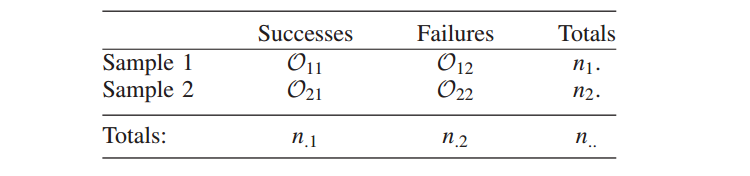
\includegraphics[width=0.7\linewidth]{fig/2x2-table}
	\caption{2 $\times$ 2 Table of Outcomes}
	\label{fig:2x2-table}
\end{figure}

\subsection{Conditional Test vs. Unconditional Test}

In many $2 \times 2$ tables, the row of a table refer to different groups, the sample size for those groups are often fixed by the sample design. Sometimes we refer rows as samples, or $X$ and refer columns as results, or $Y$.

When the marginal totals for the levels of $X$ (Samples) are fixed rather than random, a joint distribution for $X$ and $Y$ (Result) is not meaningful. We are actually more interested in the conditional distribution, $\P(Y=1|X=1)$.

As there are two outcome categories for $Y$ , the binomial
distribution applies for each conditional distribution. We assume
a binomial distribution for the sample in each row, with number
of trials equal to the fixed row total.

When there are more than two outcome categories for $Y$ , such
as (\textit{always, sometimes, never}), the multinomial distribution
applies for each conditional distribution.

To better understand this, let us consider a generic 2 $\times$ 2 contingency table obtained by inoculating 15 subjects with vaccine and 15 subjects with placebo.

% Please add the following required packages to your document preamble:
% \usepackage{multirow}
\begin{table}[H]
	\centering
	\begin{tabular}{|l|l|l|l|}
		\hline
		\multirow{2}{*}{Treatment} & \multicolumn{2}{l|}{Infection Status} & \multirow{2}{*}{Total} \\ \cline{2-3}
		& Yes             & No                  &                        \\ \hline
		Vaccine                    & $x_e$           & $15 - x_e$          & 15                     \\ \hline
		Placebo                    & $x_c$           & $15 - x_c$          & 15                     \\ \hline
		Total                      & $x_e + x_c$     & $30 - x_e -x_c$     & 30                     \\ \hline
	\end{tabular}
\end{table}

From unconditional test's perspective, the probability of observing the table is a product of two binomials. Suppose the null hypothesis is $\pi_e = \pi_c = \pi$.
\[\P(\text{Observe the Table} | \pi) = {15 \choose x_c} {15 \choose x_e} \pi^{x_c + x_e} (1 - \pi)^{30 - x_c -x_e}\]
The $p$-value is 
\[p = \sum_{T(\text{Observed Table}) \ge T(\text{Null Table})} \P(\text{Observe the Table} | \pi)\]
From the conditional test's perspective,the probability of observing the table is a product of two binomials. Suppose we observe 19 infections in total.

\[\P(\text{Observe the Table} | x_c + x_e = 19) = \frac{{15 \choose x_c} {15 \choose x_e}}{{30 \choose 19}}\]

The $p$-value is 
\[p = \sum_{T(\text{Observed Table}) \ge T(\text{Null Table})} \P(\text{Observe the Table} | x_c + x_e = 19)\]
\subsection{Assumption}
It has been shown that conditional test outperform unconditional test. So here we make $n_1$ and $n_2$ fixed then have the following assumptions.
\begin{itemize}
	\item $O_{11}$ is the number of success observed in $n_{1\cdot}$ independent Bernoulli trials, each with success probability $\pi_1$.
	\item $O_{21}$ is the number of success observed in $n_{2\cdot}$ independent Bernoulli trials, each with success probability $\pi_2$.
	\item The Bernoulli trials corresponding to sample 1 are independent of the Bernoulli trials corresponding to sample 2.
\end{itemize}

% https://www.nbi.dk/~petersen/Teaching/Stat2009/Barnard_ExactTest_TwoBinomials.pdf

\subsection{Hypothesis Test}
Given the following $2\times 2$ contingency, it is known that $n_1$ and $n_2$ are fixed. Then $n_{11}$, $n_1 - n_{11}$, $n_{21}$, and $n_2 - n_{21}$ are random variables.

\begin{figure}[H]
	\centering
	
\includegraphics[width=0.7\linewidth]{fig/2x2-table1}
	\caption{Random Variable in Contingency Table}
	\label{fig:2x2-table1}
\end{figure}

The sample proportions are $p_1 = n_{11}/ n_1$ and $p_2 = n_{21} / n_2$.

Since $n_{11} \sim \text{Binomial}(n_1, \pi_1)$, we have
\[\E p_1 = \pi_1, \Var p_1 = \frac{\pi_1 (1 - \pi_1)}{n_1}\]

Since $n_{21} \sim \text{Binomial}(n_2, p_2)$, we have
\[\E p_2 = \pi_2, \Var p_2 = \frac{\pi_2 (1 - \pi_2)}{n_2}\]

Therefore,
\[\E(p_2 - p_1) = \E p_2 - \E p_1 = \pi_2 - \pi_1\] 

Interestingly, given $n_1$ and $n_2$, the derived sample porpotion can be used to estimate the unobservable probability. The null hypothesis is constructed based on that.

\subsubsection{Approximation}
The hypothesis of interest is 
\[H_0: \pi_1 = \pi_2 = \pi\]
with the common value $\pi$ being unspecified.

We construct the test statistic based on the difference between $p_1$ and $p_2$. For Wald test, we need the mean and standard deviation of $p_1 - p_2$.
\begin{itemize}
	\item Based on null hypothesis, $\text{mean}(p_1 - p_2) = 0$.
	\item For SD, suppose $p = \frac{n_{11} + n_{21}}{n_1 + n_2}$,
	\[\text{SD}(p_1 - p_2) = \sqrt{\frac{p(1-p)}{n_1} + \frac{p(1-p)}{n_2}}\]
\end{itemize}

Therefore, we have the Wald test statistic of $p_1 - p_2$,
\[T = \frac{p_1 - p_2}{\text{SD}(p_1 - p_2)}\]

The alternative hypothesis and reject region are 
\begin{itemize}
	\item $H_1: \pi_1 > \pi_2$: Reject $H_0$ if $T \ge z_\alpha$.
	\item $H_1: \pi_1 < \pi_2$: Reject $H_0$ if $T \le z_\alpha$.
	\item $H_1: \pi_1 \neq \pi_2$: Reject $H_0$ if $|T| \ge z_{\alpha/2}$
\end{itemize}

The construction of the confidence interval for $\pi_1 - \pi_2$ is a little bit different than usual one-sample binomial distribution, where CI can be calculated by inverting the test statistic because of the duality.

The test statistic $T$ is based on the null hypothesis, where the two binomial distribution share the same $p$, while we see them as two different distribution when estimating the CI, so that we have
\[S = \sqrt{\frac{p_1(1-p_1)}{n_1} + \frac{p_2(1-p_2)}{n_2}}\]

Hence, the confidence interval for $\pi_1 - \pi_2$ is
\[p_1 - p_2 - Z_{\alpha/2} S \le \pi_1 - \pi_2 \le p_1 - p_2 + Z_{\alpha/2} S\]

\subsubsection{Notes on Alternative Hypothesis}
When choosing alternative hypothesis, by convention people choose two-sided-test, it is harder to be rejected. In other words, if the two-sided alternative hypothesis is rejected then the one-sided must be rejected.

Usually, people first use two-sided hypothesis to reject the null hypothesis, then choose the side by infering the relationship based on the data.

\subsubsection{Notes on Continuity Correction}
Whether or not to apply continuity correction is debatable. Be convention, if you decide to use continuity correction, you must report it in the paper.

If the data size is large, the continuity correction usually have no effect on the rejection of hypothesis. But when the data is small, you may reach the different conclusion of rejection. Then we need to do further simulation to exam the model.

\subsection{Action in R}
Recall that the square of normal distribution is the chi-squared distribution with one degree of freedom. So the following two calculations give the same $p$-values.

\lstinputlisting[language=R]{code/l9-exp1.R}

Probabilities of success in R without continuity correction.
\lstinputlisting[language=R]{code/l9-exp2.R}
Probabilities of success in R with continuity correction.
\lstinputlisting[language=R]{code/l9-exp3.R}